\shorthandoff{:!}\begin{circuitikz}[scale=1]
%	\draw [help lines, step=0.5cm] (0.25,0) grid (7.75,5);
	\node [below] at (4, 0.05) {$T_b$};
	\fill [pattern = north east lines] (2.5,0.05) rectangle (5.5,0.25);
	\draw [brown, line width = 5] (4,0.25) -- (4,1.75);
	\draw [thick] (2.5,0.25) -- (5.5,0.25);
	\draw [brown, line width = 5] (3.25, 2.5) -- (1.75, 2.5);
	\draw [brown, line width = 5] (4.75, 2.5) -- (6.25, 2.5);
	\node [right] at (4, 1)	{$G_{pb}$};
	\node [left, red] at (4, 1)	{$P_{ap}$};
	\node [below] at (2.5, 2.5)	{$G_{ap}$};
	\node [above, red] at (2.5, 2.5)	{$P_{pb}$};
	\node [below] at (5.5, 2.5)	{$G_{ep}$};
	\node [above, red] at (5.5, 2.5)	{$P_{ep}$};
	\draw [fill=yellow] (3.25, 1.75) rectangle (4.75, 3.25);
	\node at (4, 2.5) {$T_p$};
	\draw [fill=orange] (1.75, 1.75) rectangle (0.25, 3.25);
	\node at (1, 2.5) {$T_a$};
	\draw [fill=cyan] (6.25, 1.75) rectangle (7.75, 3.25);
	\node at (7, 2.5) {$T_e$};
	\node [anchor=south, inner sep=0] at (1, 3.5)
    	{\resizebox{2cm}{!}{% This file was created by matplotlib2tikz v0.6.10.
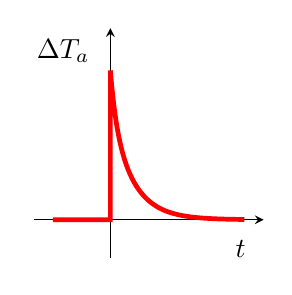
\begin{tikzpicture}

\begin{axis}[
ticks=none,
xmin=-0.2, xmax=0.4,
ymin=-0.5e-07, ymax=2.5e-07,
axis x line=center,
axis y line=center,
every axis x label/.style={at={(ticklabel cs:0.9)}, below=4pt},
every axis y label/.style={at={(ticklabel cs:0.9)}, left=4pt},
xlabel={$t$},
ylabel={$\Delta T_a$},
width=4.5cm,
height=4.5cm
]
\addplot [line width = 1.7pt, red]
table {%
-0.15 0
1e-08 0
0 1.94905773450583e-07
0.00353535353535354 1.75086151002447e-07
0.00707070707070707 1.58214334725911e-07
0.0106060606060606 1.4370498349366e-07
0.0141414141414141 1.31131841539708e-07
0.0176767676767677 1.20154073651191e-07
0.0212121212121212 1.10498558052284e-07
0.0247474747474747 1.01945886553252e-07
0.0282828282828283 9.43192935859211e-08
0.0318181818181818 8.74758993005682e-08
0.0353535353535354 8.1299781085828e-08
0.0388888888888889 7.56964899078769e-08
0.0424242424242424 7.05887084549368e-08
0.045959595959596 6.59128117256344e-08
0.0494949494949495 6.16161409749693e-08
0.053030303030303 5.76548416413408e-08
0.0565656565656566 5.39921472429897e-08
0.0601010101010101 5.05970160062528e-08
0.0636363636363636 4.74430465564955e-08
0.0671717171717172 4.45076144595586e-08
0.0707070707070707 4.17711836111647e-08
0.0742424242424242 3.92167561164711e-08
0.0777777777777778 3.68294319208594e-08
0.0813131313131313 3.45960554718693e-08
0.0848484848484848 3.25049314471608e-08
0.0883838383838384 3.05455953401098e-08
0.0919191919191919 2.8708627662862e-08
0.0954545454545454 2.69855028720667e-08
0.098989898989899 2.53684659759339e-08
0.102525252525253 2.38504312460595e-08
0.106060606060606 2.24248986152695e-08
0.10959595959596 2.10858842580303e-08
0.113131313131313 1.98278625736718e-08
0.116666666666667 1.86457173650087e-08
0.12020202020202 1.75347004576861e-08
0.123737373737374 1.64903963638234e-08
0.127272727272727 1.55086918770988e-08
0.130808080808081 1.45857497109756e-08
0.134343434343434 1.37179854696812e-08
0.137878787878788 1.29020473825878e-08
0.141414141414141 1.21347983445272e-08
0.144949494949495 1.14132998934018e-08
0.148484848484848 1.07347978270466e-08
0.152020202020202 1.00967092174591e-08
0.155555555555556 9.49661062525964e-09
0.159090909090909 8.93222735294378e-09
0.162626262626263 8.40142360402661e-09
0.166161616161616 7.9021934380375e-09
0.16969696969697 7.43265242968028e-09
0.173232323232323 6.99102995525483e-09
0.176767676767677 6.57566204137687e-09
0.18030303030303 6.18498472071477e-09
0.183838383838384 5.81752784734487e-09
0.187373737373737 5.4719093307749e-09
0.190909090909091 5.14682975298612e-09
0.194444444444444 4.84106733722839e-09
0.197979797979798 4.5534732409492e-09
0.201515151515152 4.28296714829148e-09
0.205050505050505 4.02853314017069e-09
0.208585858585859 3.78921582212947e-09
0.212121212121212 3.56411669204082e-09
0.215656565656566 3.35239073134553e-09
0.219191919191919 3.15324320491336e-09
0.222727272727273 2.96592665584594e-09
0.226262626262626 2.78973808262336e-09
0.22979797979798 2.62401628695844e-09
0.233333333333333 2.46813938158316e-09
0.236868686868687 2.32152244796522e-09
0.24040404040404 2.18361533465225e-09
0.243939393939394 2.05390058757701e-09
0.247474747474747 1.93189150423773e-09
0.251010101010101 1.81713030419968e-09
0.254545454545455 1.70918640885407e-09
0.258080808080808 1.6076548238223e-09
0.261616161616162 1.51215461781191e-09
0.265151515151515 1.42232749211878e-09
0.268686868686869 1.3378364353309e-09
0.272222222222222 1.2583644581251e-09
0.275757575757576 1.18361340336156e-09
0.279292929292929 1.11330282697358e-09
0.282828282828283 1.04716894542388e-09
0.286363636363636 9.84963645754594e-10
0.28989898989899 9.26453554498324e-10
0.293434343434343 8.71419161942022e-10
0.296969696969697 8.19653998446613e-10
0.30050505050505 7.70963859722854e-10
0.304040404040404 7.25166078149621e-10
0.307575757575758 6.82088837395062e-10
0.311111111111111 6.41570527764773e-10
0.314646464646465 6.03459139854875e-10
0.318181818181818 5.67611694232354e-10
0.321717171717172 5.33893705000791e-10
0.325252525252525 5.02178675237199e-10
0.328787878787879 4.72347622405636e-10
0.332323232323232 4.44288631966024e-10
0.335858585858586 4.17896437502591e-10
0.339393939393939 3.93072025796083e-10
0.342929292929293 3.69722265357532e-10
0.346464646464646 3.47759557029615e-10
0.35 3.27101505344391e-10
};
\end{axis}

\end{tikzpicture}}};
    \node [anchor=south, inner sep=0] at (4, 3.5)
    	{\resizebox{2cm}{!}{% This file was created by matplotlib2tikz v0.6.10.
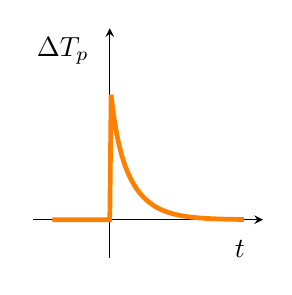
\begin{tikzpicture}

\definecolor{color0}{rgb}{1,0.647058823529412,0}


\begin{axis}[
ticks=none,
xmin=-0.2, xmax=0.4,
ymin=-0.5e-07, ymax=2.5e-07,
axis x line=center,
axis y line=center,
every axis x label/.style={at={(ticklabel cs:0.9)}, below=4pt},
every axis y label/.style={at={(ticklabel cs:0.9)}, left=4pt},
xlabel={$t$},
ylabel={$\Delta T_p$},
width=4.5cm,
height=4.5cm
]
\addplot [line width = 1.7pt, orange]
table {%
-0.15 0
1e-08 0
0 6.96368541805659e-24
0.00353535353535354 1.63176399143611e-07
0.00707070707070707 1.48010174769528e-07
0.0106060606060606 1.34895295323391e-07
0.0141414141414141 1.23468086776223e-07
0.0176767676767677 1.13437308330477e-07
0.0212121212121212 1.04569165237934e-07
0.0247474747474747 9.6675457798133e-08
0.0282828282828283 8.96042081124974e-08
0.0318181818181818 8.32322445633661e-08
0.0353535353535354 7.74593332500688e-08
0.0388888888888889 7.22035319129691e-08
0.0424242424242424 6.73975100378826e-08
0.045959595959596 6.29856326697683e-08
0.0494949494949495 5.89216479870297e-08
0.053030303030303 5.51668522742115e-08
0.0565656565656566 5.16886324595516e-08
0.0601010101010101 4.8459307338149e-08
0.0636363636363636 4.54552051530634e-08
0.0671717171717172 4.26559282807991e-08
0.0707070707070707 4.00437660952089e-08
0.0742424242424242 3.76032252420987e-08
0.0777777777777778 3.53206530016271e-08
0.0813131313131313 3.31839345070543e-08
0.0848484848484848 3.11822486108937e-08
0.0883838383838384 2.93058703676763e-08
0.0919191919191919 2.75460106137664e-08
0.0954545454545454 2.58946851090798e-08
0.098989898989899 2.43446072738405e-08
0.102525252525253 2.28890997930618e-08
0.106060606060606 2.15220213413162e-08
0.10959595959596 2.02377054550822e-08
0.113131313131313 1.90309091926043e-08
0.116666666666667 1.78967697058042e-08
0.12020202020202 1.68307672321937e-08
0.123737373737374 1.58286933182089e-08
0.127272727272727 1.48866233256637e-08
0.130808080808081 1.40008924633649e-08
0.134343434343434 1.31680747367947e-08
0.137878787878788 1.23849643284248e-08
0.141414141414141 1.16485590162039e-08
0.144949494949495 1.0956045313217e-08
0.148484848484848 1.0304785071529e-08
0.152020202020202 9.69230334102103e-09
0.155555555555556 9.11627731213953e-09
0.159090909090909 8.57452620193543e-09
0.162626262626263 8.06500196714538e-09
0.166161616161616 7.58578074763144e-09
0.16969696969697 7.13505495923382e-09
0.173232323232323 6.71112596779503e-09
0.176767676767677 6.31239728640301e-09
0.18030303030303 5.93736824626804e-09
0.183838383838384 5.58462809848333e-09
0.187373737373737 5.25285050953076e-09
0.190909090909091 4.94078841802559e-09
0.194444444444444 4.64726922404115e-09
0.197979797979798 4.37119028557055e-09
0.201515151515152 4.111514699389e-09
0.205050505050505 3.86726734587531e-09
0.208585858585859 3.63753117931072e-09
0.212121212121212 3.4214437468602e-09
0.215656565656566 3.21819392090423e-09
0.219191919191919 3.02701883066689e-09
0.222727272727273 2.84720098021137e-09
0.226262626262626 2.67806554087111e-09
0.22979797979798 2.51897780707433e-09
0.233333333333333 2.36934080531901e-09
0.236868686868687 2.2285930467763e-09
0.24040404040404 2.09620641465547e-09
0.243939393939394 1.97168417806043e-09
0.247474747474747 1.85455912461491e-09
0.251010101010101 1.74439180463596e-09
0.254545454545455 1.64076888009906e-09
0.258080808080808 1.54330157206693e-09
0.261616161616162 1.45162420065171e-09
0.265151515151515 1.36539281194944e-09
0.268686868686869 1.28428388672967e-09
0.272222222222222 1.20799312598366e-09
0.275757575757576 1.13623430873391e-09
0.279292929292929 1.06873821778733e-09
0.282828282828283 1.00525162937641e-09
0.286363636363636 9.45536362877567e-10
0.28989898989899 8.89368387025501e-10
0.293434343434343 8.36536979257968e-10
0.296969696969697 7.86843935027003e-10
0.30050505050505 7.4010282410245e-10
0.304040404040404 6.96138291071478e-10
0.307575757575758 6.54785397404927e-10
0.311111111111111 6.15889002618282e-10
0.314646464646465 5.79303182202572e-10
0.318181818181818 5.44890680139068e-10
0.321717171717172 5.12522393941935e-10
0.325252525252525 4.82076890295391e-10
0.328787878787879 4.53439949467044e-10
0.332323232323232 4.26504136787296e-10
0.335858585858586 4.01168399586413e-10
0.339393939393939 3.77337688076548e-10
0.342929292929293 3.5492259875595e-10
0.346464646464646 3.33839038997186e-10
0.35 3.14007911560752e-10
};
\end{axis}

\end{tikzpicture}}};	
    \node [anchor=south, inner sep=0] at (7, 3.5)
    	{\resizebox{2cm}{!}{% This file was created by matplotlib2tikz v0.6.10.
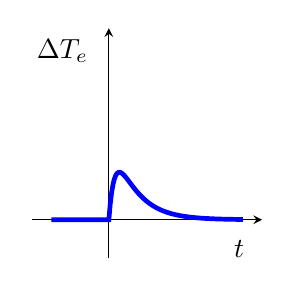
\begin{tikzpicture}

\begin{axis}[
ticks=none,
xmin=-0.2, xmax=0.4,
ymin=-0.5e-07, ymax=2.5e-07,
axis x line=center,
axis y line=center,
every axis x label/.style={at={(ticklabel cs:0.9)}, below=4pt},
every axis y label/.style={at={(ticklabel cs:0.9)}, left=4pt},
xlabel={$t$},
ylabel={$\Delta T_e$},
width=4.5cm,
height=4.5cm
]
\addplot [line width = 1.7pt, blue]
table {%
-0.15 0
1e-08 0
0 5.15986218822629e-23
0.00353535353535354 2.02319742455945e-08
0.00707070707070707 3.50283638973746e-08
0.0106060606060606 4.55829895717481e-08
0.0141414141414141 5.2854683483701e-08
0.0176767676767677 5.75967408445595e-08
0.0212121212121212 6.04003591661948e-08
0.0247474747474747 6.17289341324563e-08
0.0282828282828283 6.19451332621564e-08
0.0318181818181818 6.13322662511764e-08
0.0353535353535354 6.0111151566108e-08
0.0388888888888889 5.84534266690334e-08
0.0424242424242424 5.64920500734984e-08
0.045959595959596 5.4329586121974e-08
0.0494949494949495 5.20447391339915e-08
0.053030303030303 4.96975054505508e-08
0.0565656565656566 4.73332344043295e-08
0.0601010101010101 4.49858280406682e-08
0.0636363636363636 4.26802610766907e-08
0.0671717171717172 4.04345644105182e-08
0.0707070707070707 3.82613853431711e-08
0.0742424242424242 3.6169213865249e-08
0.0777777777777778 3.41633455563404e-08
0.0813131313131313 3.22466367949145e-08
0.0848484848484848 3.04200962489964e-08
0.0883838383838384 2.86833473567554e-08
0.0919191919191919 2.70349891927568e-08
0.0954545454545454 2.54728773405602e-08
0.098989898989899 2.39943418321705e-08
0.102525252525253 2.25963556141392e-08
0.106060606060606 2.12756641571379e-08
0.10959595959596 2.00288845812559e-08
0.113131313131313 1.88525808972803e-08
0.116666666666667 1.77433205654116e-08
0.12020202020202 1.66977164687768e-08
0.123737373737374 1.571245752772e-08
0.127272727272727 1.4784330493241e-08
0.130808080808081 1.39102349154358e-08
0.134343434343434 1.30871928548508e-08
0.137878787878788 1.23123545671688e-08
0.141414141414141 1.15830011255645e-08
0.144949494949495 1.0896544735358e-08
0.148484848484848 1.02505273303853e-08
0.152020202020202 9.64261791040749e-09
0.155555555555556 9.07060897650632e-09
0.159090909090909 8.53241234089511e-09
0.162626262626263 8.02605452431492e-09
0.166161616161616 7.54967190452406e-09
0.16969696969697 7.10150574045727e-09
0.173232323232323 6.67989716615275e-09
0.176767676767677 6.2832822247284e-09
0.18030303030303 5.91018699411838e-09
0.183838383838384 5.55922284183937e-09
0.187373737373737 5.2290818348624e-09
0.190909090909091 4.91853232202482e-09
0.194444444444444 4.62641469977975e-09
0.197979797979798 4.35163736701518e-09
0.201515151515152 4.09317287084003e-09
0.205050505050505 3.85005424236218e-09
0.208585858585859 3.62137151936202e-09
0.212121212121212 3.40626845122712e-09
0.215656565656566 3.20393938043e-09
0.219191919191919 3.01362629409614e-09
0.222727272727273 2.83461603874513e-09
0.226262626262626 2.66623769102869e-09
0.22979797979798 2.50786007718652e-09
0.233333333333333 2.35888943395577e-09
0.236868686868687 2.21876720377107e-09
0.24040404040404 2.08696795725728e-09
0.243939393939394 1.96299743622671e-09
0.247474747474747 1.84639071063342e-09
0.251010101010101 1.73671044319756e-09
0.254545454545455 1.63354525568494e-09
0.258080808080808 1.53650819110403e-09
0.261616161616162 1.44523526636046e-09
0.265151515151515 1.359384110183e-09
0.268686868686869 1.27863268140426e-09
0.272222222222222 1.20267806293949e-09
0.275757575757576 1.13123532705958e-09
0.279292929292929 1.06403646779599e-09
0.282828282828283 1.00082939654757e-09
0.286363636363636 9.41376997180387e-10
0.28989898989899 8.85456237122462e-10
0.293434343434343 8.32857331155583e-10
0.296969696969697 7.83382954796269e-10
0.30050505050505 7.36847504337837e-10
0.304040404040404 6.93076400795766e-10
0.307575757575758 6.51905435159421e-10
0.311111111111111 6.13180152505136e-10
0.314646464646465 5.76755272669063e-10
0.318181818181818 5.42494145313467e-10
0.321717171717172 5.10268237347692e-10
0.325252525252525 4.79956650785216e-10
0.328787878787879 4.51445669231489e-10
0.332323232323232 4.24628331303897e-10
0.335858585858586 3.9940402938568e-10
0.339393939393939 3.75678132210213e-10
0.342929292929293 3.53361629861074e-10
0.346464646464646 3.32370799857171e-10
0.35 3.12626893071057e-10
};
\end{axis}

\end{tikzpicture}}};
    	
\end{circuitikz}\shorthandon{:!}